% Options for packages loaded elsewhere
\PassOptionsToPackage{unicode}{hyperref}
\PassOptionsToPackage{hyphens}{url}
%
\documentclass[
]{article}
\usepackage{amsmath,amssymb}
\usepackage{lmodern}
\usepackage{iftex}
\ifPDFTeX
  \usepackage[T1]{fontenc}
  \usepackage[utf8]{inputenc}
  \usepackage{textcomp} % provide euro and other symbols
\else % if luatex or xetex
  \usepackage{unicode-math}
  \defaultfontfeatures{Scale=MatchLowercase}
  \defaultfontfeatures[\rmfamily]{Ligatures=TeX,Scale=1}
\fi
% Use upquote if available, for straight quotes in verbatim environments
\IfFileExists{upquote.sty}{\usepackage{upquote}}{}
\IfFileExists{microtype.sty}{% use microtype if available
  \usepackage[]{microtype}
  \UseMicrotypeSet[protrusion]{basicmath} % disable protrusion for tt fonts
}{}
\makeatletter
\@ifundefined{KOMAClassName}{% if non-KOMA class
  \IfFileExists{parskip.sty}{%
    \usepackage{parskip}
  }{% else
    \setlength{\parindent}{0pt}
    \setlength{\parskip}{6pt plus 2pt minus 1pt}}
}{% if KOMA class
  \KOMAoptions{parskip=half}}
\makeatother
\usepackage{xcolor}
\usepackage[margin=1in]{geometry}
\usepackage{longtable,booktabs,array}
\usepackage{calc} % for calculating minipage widths
% Correct order of tables after \paragraph or \subparagraph
\usepackage{etoolbox}
\makeatletter
\patchcmd\longtable{\par}{\if@noskipsec\mbox{}\fi\par}{}{}
\makeatother
% Allow footnotes in longtable head/foot
\IfFileExists{footnotehyper.sty}{\usepackage{footnotehyper}}{\usepackage{footnote}}
\makesavenoteenv{longtable}
\usepackage{graphicx}
\makeatletter
\def\maxwidth{\ifdim\Gin@nat@width>\linewidth\linewidth\else\Gin@nat@width\fi}
\def\maxheight{\ifdim\Gin@nat@height>\textheight\textheight\else\Gin@nat@height\fi}
\makeatother
% Scale images if necessary, so that they will not overflow the page
% margins by default, and it is still possible to overwrite the defaults
% using explicit options in \includegraphics[width, height, ...]{}
\setkeys{Gin}{width=\maxwidth,height=\maxheight,keepaspectratio}
% Set default figure placement to htbp
\makeatletter
\def\fps@figure{htbp}
\makeatother
\setlength{\emergencystretch}{3em} % prevent overfull lines
\providecommand{\tightlist}{%
  \setlength{\itemsep}{0pt}\setlength{\parskip}{0pt}}
\setcounter{secnumdepth}{5}
\newlength{\cslhangindent}
\setlength{\cslhangindent}{1.5em}
\newlength{\csllabelwidth}
\setlength{\csllabelwidth}{3em}
\newlength{\cslentryspacingunit} % times entry-spacing
\setlength{\cslentryspacingunit}{\parskip}
\newenvironment{CSLReferences}[2] % #1 hanging-ident, #2 entry spacing
 {% don't indent paragraphs
  \setlength{\parindent}{0pt}
  % turn on hanging indent if param 1 is 1
  \ifodd #1
  \let\oldpar\par
  \def\par{\hangindent=\cslhangindent\oldpar}
  \fi
  % set entry spacing
  \setlength{\parskip}{#2\cslentryspacingunit}
 }%
 {}
\usepackage{calc}
\newcommand{\CSLBlock}[1]{#1\hfill\break}
\newcommand{\CSLLeftMargin}[1]{\parbox[t]{\csllabelwidth}{#1}}
\newcommand{\CSLRightInline}[1]{\parbox[t]{\linewidth - \csllabelwidth}{#1}\break}
\newcommand{\CSLIndent}[1]{\hspace{\cslhangindent}#1}
\ifLuaTeX
  \usepackage{selnolig}  % disable illegal ligatures
\fi
\IfFileExists{bookmark.sty}{\usepackage{bookmark}}{\usepackage{hyperref}}
\IfFileExists{xurl.sty}{\usepackage{xurl}}{} % add URL line breaks if available
\urlstyle{same} % disable monospaced font for URLs
\hypersetup{
  pdftitle={Expected travel time delay and weather conditions},
  pdfauthor={Maria Osipenko},
  hidelinks,
  pdfcreator={LaTeX via pandoc}}

\title{Expected travel time delay and weather conditions}
\author{Maria Osipenko}
\date{2023-07-21}

\usepackage{amsthm}
\newtheorem{theorem}{Theorem}[section]
\newtheorem{lemma}{Lemma}[section]
\newtheorem{corollary}{Corollary}[section]
\newtheorem{proposition}{Proposition}[section]
\newtheorem{conjecture}{Conjecture}[section]
\theoremstyle{definition}
\newtheorem{definition}{Definition}[section]
\theoremstyle{definition}
\newtheorem{example}{Example}[section]
\theoremstyle{definition}
\newtheorem{exercise}{Exercise}[section]
\theoremstyle{definition}
\newtheorem{hypothesis}{Hypothesis}[section]
\theoremstyle{remark}
\newtheorem*{remark}{Remark}
\newtheorem*{solution}{Solution}
\begin{document}
\maketitle

\hypertarget{background}{%
\section{Background}\label{background}}

Models of optimal departure time choice contain frequently a scheduling component, where the disutility or costs from early or late arrival weighted by preference parameters come into play. The vast majority of those models builds upon an asymmetric linear scheduling part (Fosgerau and Karlström (2010), Zhang and Homem-de-Mello (2017), Guo et al. (2017), Li (2019), Jin (2020)). Taking the utility approach of Fosgerau and Karlström (2010), one ahs:

\begin{equation}U_1(d,T) = -\{\alpha T + \beta(d-T)\mathbf 1_{T<d} + \gamma (T-d)\mathbf 1_{T\geq d}\}, \label{eq:u1}
\end{equation}

where \(T\) is random travel time with cumulative distribution function \(F\), the preferred arrival time is normalized to \(0\), and \(-d\), \(d>0\) is the departure time to choose.
The optimal departure time has been shown to be equal to \(d_1^* = \mu + \sigma F^{-1}\left(\frac{\gamma}{\beta+\gamma}\right)\) in Fosgerau and Karlström (2010). This type of utility comes with the assumption of strictly increasing cumulative distribution function \(F\) of the travel time \(T\), such that the inverse \(F^{-1}\left(\frac{\gamma}{\beta+\gamma}\right)\) for all possible preference parametrizations \(\beta\) and \(\gamma\) exists. That is, this scheduling approach does not work in case of discrete travel time distributions or mixture distributions with a discrete component as in de Palma and Picard (2006). The authors in de Palma and Picard (2006) sensibly model the travel time distribution as a mixture of a continuous part on bad days and a discrete component on good days. For their analysis of risk preferences and information value, they use the classical mean-variance and mean-deviation utility functions, as well as standard utilities with constant absolute and constant relative risk aversion. Later in the generalized setting, de Palma, Lindsey, and Picard (2012) assume a differentiable utility function, which rules out the specification in \eqref{eq:u1}. The later, however arguably describes the scheduling choice more ``authentically''.

In this paper, we propose an alternative specification of the scheduling part. Concretely, we define:
\begin{equation}U_2(d,T) = -\{\alpha T + \beta(d-T)^2\mathbf 1_{T<d} + \gamma (T-d)^2\mathbf 1_{T\geq d}\} \label{eq:u2}
\end{equation}
with asymmetric \emph{quadratic} loss on the early or late arrival. In this preferences formulation, the marginal disutility increases along with the delay magnitude, which may describe the preferences of at least some commuters in a more consistent way. In fact, this continuously differentiable preference specification fulfill the assumptions of Smith (1984) and Daganzo (1985) for existence and uniqueness of equilibrium in a single bottleneck model. It also satisfies the requirement of de Palma, Lindsey, and Picard (2012) and their equilibrium analysis with risk aversion and information value.

It turns out, that both preference specifications in \eqref{eq:u1} and \eqref{eq:u2} share the property, that the optimal departure time choices correspond to specific \emph{tail indices} of the travel time distribution. For the first specification in \eqref{eq:u1}, these are the \emph{quantiles} and for the second specification in \eqref{eq:u2}, these are the \emph{expectiles} of the travel time \(T\). The asymmetric quadratic version of the scheduling preferences and the fact, the the solutions to the expected utility maximization problem are quantiles and expectiles respectively seem to have been left unraised explicitly, in the previous literature.\footnote{Fosgerau and Karlström (2010) do mention that the distribution of standardised travel time enter the optimal departure time through its quantile.} Moreover, both types of scheduling preferences are related to each other via the quantile-expectile correspondence (Jones (1994)), whilst the second version in \eqref{eq:u2} describes a richer class of preferences compared to the first one.

In this paper, we analyse and compare the two utility specifications of scheduling preferences: the linear one in \eqref{eq:u1} and the quadratic one in \eqref{eq:u2}, where the later ``cures'' the deficiencies of the first one. That is, in the next section, we show that the optimal departure times are quantiles for the linear and expectiles for the quadratic case. We also show that the two utility specifications are linked through the concept of quantile-expectile correspondence and demonstrate, that the new asymmetric quadratic class is a richer one, in the sense that it covers the preferences in \eqref{eq:u1} as a special case. We derive the travel time reliability ratios to quantify the value of travel time reliability for both specifications in section 3. Using the travel time data of Montreal, we compare in section 4 the optimal choices corresponding to the two utility specifications and the resulting travel time reliability ratios based on the fitted mixture distribution with three beta distribution components. Finally, we conclude and discuss further research directions.

\hypertarget{asymmetric-scheduling-preferences}{%
\section{Asymmetric scheduling preferences}\label{asymmetric-scheduling-preferences}}

Consider a planer with utility function depending on random travel time \(T\) with realizations \(t\in\mathbb R_+\) and on the departure time \(-d\) for \(d>0\) with the preferred arrival time normalized to \(0\). According to the scheduling approach of Fosgerau and Karlström (2010), as already specified in \eqref{eq:u1}:

\[U_1(d,T) = -\{\alpha T + \beta(d-T)\mathbf 1_{T<d} + \gamma (T-d)\mathbf 1_{T\geq d}\}\]

for \(\gamma>\beta>0\) for an equilibrium state to be reached (K. Small (1982), K. A. Small (2015)). In this formulation, both early and late arrivals increase the disutility of the planer in a \textbf{linear} manner with the marginal disutility of early arrival being equal to \(\beta\) and the marginal disutility of late arrival being equal to \(\gamma\). Note, that the utility decrease is asymmetric regarding the type of delay (early or late).

The asymmetric linear loss may be unrealistic in many situations, because marginal disutility of early delays or late delays is constant and does not depend on the magnitude of the delay. Bogers et al. (2006) for instance find that extremely long travel times influence significantly the route choice. When the marginal disutility increases along with the delay magnitude and an asymmetric \textbf{quadratic} loss would describe such preferences in a more consistent way. In fact, such specification of the planer utility function even simplifies the computation of the optimal departure time, as we show later. The asymmetric quadratic version \(U_2(d,T)\) mentioned previously in \eqref{eq:u2} reads:

\[U_2(d,T) = -\{\alpha T + \beta(d-T)^2\mathbf 1_{T<d} + \gamma (T-d)^2\mathbf 1_{T\geq d}\}\]
The marginal disutility of early arrival (\(d>t\)) becomes \(\beta (d-t)\) and the marginal disutility of late arrival (\(d\leq t\)) becomes \(\gamma (t-d)\).

The later formulation of preferences in \eqref{eq:u2} has the advantage of being differentiable with respect to \(d\), which is a condition of uniqueness of the resulting equilibrium distribution of arrivals at a single bottleneck model (Daganzo (1985)). Moreover, both utility functions are reformulations of cost functions in departure time choice problems in single bottlenecks as in Lindsey (2004).

We assume, that planer maximizes her expected utility, which is in this case (\(\mathbb E(\cdot)\) denotes the expectation with respect to the distribution function of \(T\), \(F\)):

\begin{itemize}
\item
  \textbf{linear asymmetric case}
  \begin{equation}\mathbb EU_1(d,T) = -\left[\alpha \mathbb ET + \beta\mathbb E\left\{(d-T)\mathbf 1_{T<d} \right\}+ \gamma \mathbb E\left\{(T-d)\mathbf 1_{T\geq d}\right\}\right]. \label{eq:eu1}
  \end{equation}
\item
  \textbf{quadratic asymmetric case}
  \begin{equation}
  \mathbb EU_2(d,T) = -\left[\alpha \mathbb ET + \beta\mathbb E\left\{(d-T)^2\mathbf 1_{T<d} \right\}+ \gamma \mathbb E\left\{(T-d)^2\mathbf 1_{T\geq d}\right\}\right]. \label{eq:eu2}
  \end{equation}
\end{itemize}

Both utility formulations fall under the mean-dispersion framework (Engelson and Fosgerau (2016)) with different notions of dispersion used. For \(\beta=\gamma\), \eqref{eq:eu1} corresponds to a symmetric mean-absolute deviation utility and the optimal choice \(d^*_1\) corresponds to the median of the travel times. For \(\gamma>\beta\) it remains asymmetric, and the second term in the maximized utility \(\mathbb EU^*_1(d_1^*,T)\) is an asymmetric version of absolute deviation termed in Tran et al. (2019) as the \textbf{\(\tau\)-deviation} (asymmetrically weighted deviation around the \textbf{\(\tau\)-quantile}). Similarly, for \(\beta=\gamma\), \eqref{eq:eu2} becomes \(\mathbb EU_2(d,T) = -\left[\alpha \mathbb ET + \beta\mathbb E\left\{(T-d)^2\right\}\right]\),
which is maximized for \(d_2^* = \mathbb ET\). Hence we recover the classical mean-variance utility \(\mathbb EU^*_2(d_2^*,T)\) used by Jackson and Jucker (1982). For \(\gamma>\beta\) the second term in the maximized utility \(\mathbb EU^*_2(d_2^*,T)\) is a generalized version of the variance - \textbf{the \(\tau\)-variance} - around a certain tail index - \textbf{the \(\tau\)-expectile}.

\begin{verbatim}
## The legacy packages maptools, rgdal, and rgeos, underpinning this package
## will retire shortly. Please refer to R-spatial evolution reports on
## https://r-spatial.org/r/2023/05/15/evolution4.html for details.
## This package is now running under evolution status 0
\end{verbatim}

\hypertarget{optimal-departure-time-choice-under-asymmetric-scheduling-preferences}{%
\section{Optimal departure time choice under asymmetric scheduling preferences}\label{optimal-departure-time-choice-under-asymmetric-scheduling-preferences}}

In this section, we show that the optimal departure time turns to be equal to a certain quantile (see Koenker and Bassett (1978)) in case of \(U_1(d,T)\) and a certain expectile (see Newey and Powell (1987)) for \(U_2(d,T)\) of the travel time distribution. The particular quantile or expectile levels depend on the asymmetry parameter (\(\beta\) and \(\gamma\)) of planer's utility function. We, therefore briefly review the concepts of quantiles and expectiles in the following.

\hypertarget{quantiles-and-expectiles}{%
\subsection{Quantiles and expectiles}\label{quantiles-and-expectiles}}

Quantiles and expectiles are real numbers which describe a distribution of a real random variable \(X\). They generalize the median and the mean respectively to their asymmetric versions via the asymmetry index \(\tau\in(0,1)\). For a suitable set of such indices \(\tau\in(0,1)\) the associated sets of either quantiles \(\{q_\tau(X)\}_{\tau\in(0,1)}\) or expectiles \(\{e_\tau(X)\}_{\tau\in(0,1)}\) are capable of representing the entire distribution of a random variable.

Both quantiles and expectiles can be viewed as minimizers of expectations of asymmetric norms (see e.g. Tran et al. (2019)):
\begin{align}
\min_{c\in\mathbb R}\mathbb E_{F_X}||X-c||^a_{a,\tau}, \text{ for } a\in\{1,2\}, \label{eq:asnorm}
\end{align}
where \(||x||^a_{a,\tau}=|x|^a\cdot\{\tau\mathbf 1_{x\geq 0}+(1-\tau)\mathbf 1_{x<0}\}\) is the asymmetric norm for \(x\in\mathbb R\).
That is, the \(\tau\)-quantile solves \(q_\tau(X) = \arg\min_{q\in\mathbb R}\mathbb E_{F_X}||X-q||^1_{1,\tau}\) whereas the \(\tau\)-expectile solves \(e_\tau(X) = \arg\min_{e\in\mathbb R}\mathbb E_{F_X}||X-e||^2_{2,\tau}\).

Expectiles are uniquely defined for random variables with finite expectations, whereas for quantiles to be unique, we need a strictly increasing cumulative distribution function \(F\). This creates difficulties in treating e.g.~discrete distributions as the following example shows.

\begin{example}[Quantiles and expectiles of a two-value travel time distribution]
\protect\hypertarget{exm:ddqande}{}\label{exm:ddqande}Consider random travel time \(T\) with two values: \(t_1\) with probability \(p\) and \(t_2\), \(t_2-t_1>0\) with probability \(1-p\)\footnote{For instance, de Palma, Lindsey, and Picard (2012) specify in this way the distribution of travel times on an uncertain route intheir analysis.}. For example, on a ideal road link without congestion two speed regimes hold depending on whether the road surface is wet or not (or there is fog or not). Then \(1-p\) could be the probability of wet surface or the probability of rain.

Since \(\mathbb P(T\leq t) = 0\) for \(t\in(-\infty,t_1)\), for any \(\tau\in (0,p]\) the \(\tau\)-quantile is any number in the range \([0,t)\). Likewise, since \(\mathbb P(T\leq t) = p\) for \(t\in[t_1,t_2)\) and for any \(\tau \in(p,1)\) it is any number in the range \([t_1,t_2)\). It is unclear whether and how much the \(\tau\)-quantile is affected by a change in \(p\).

In case of expectiles using formulas (18) and (19) in Holzmann and Klar (2015) we have:

\[e_\tau = \frac{(1-\tau)t_1p+ \tau t_2(1-p)}{(1-\tau)p + \tau(1-p)}\]
which is continuous and strictly increasing in \(\tau\) (see Figure \ref{fig:figex1}).

\begin{figure}
\centering
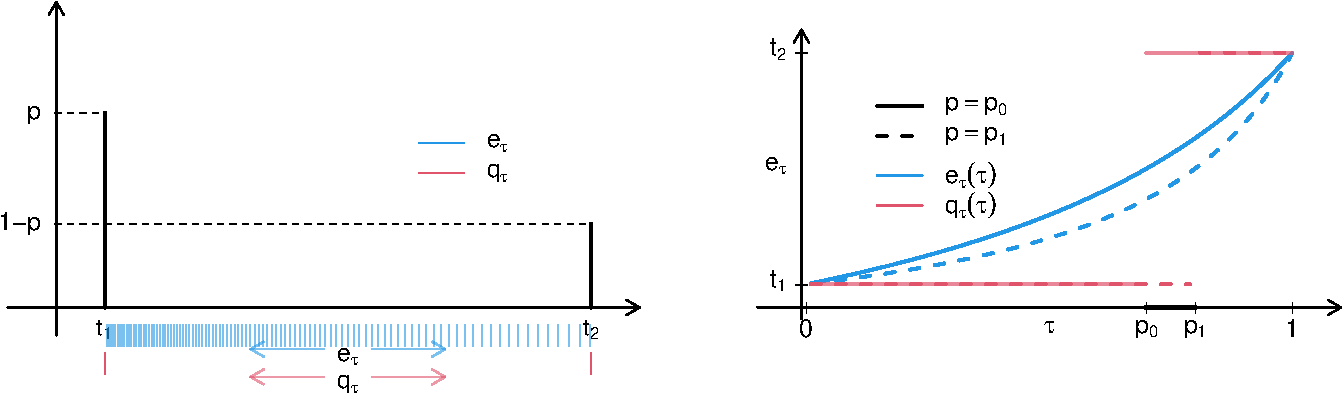
\includegraphics{paper_new_files/figure-latex/figex1-1.pdf}
\caption{\label{fig:figex1}Inverse expectile function and expectile values (below the \(x\)-axis) for a grid of \$ au\$-values in case of a two-value discrete distribution.}
\end{figure}

Since \(\frac{\partial e_\tau}{\partial l} = \tau(1-p)>0\) it is also an increasing function of \(l\). Since \(\frac{\partial e_\tau}{\partial p} =(-l)\cdot \frac{ \tau (1-\tau)} {\{\tau+p (1-2\tau )\}^2} <0\) \(e_\tau\) decreases in \(p\) or equivalent it increases in \(1-p\) (see Figure \ref{fig:figex11}).
\end{example}

\begin{figure}
\centering
\includegraphics{paper_new_files/figure-latex/figex11-1.pdf}
\caption{\label{fig:figex11}Expectile function for a two-value discrete distribution and changing \(p\).}
\end{figure}

In the example above, we derive an explicit expression for \(e_\tau\). However, this is not always possible and \(e_\tau\) is represented in an implicit functional form based on the first order condition of \eqref{eq:asnorm} for \(a=2\):

\begin{align}
\tau\mathbb E\{|Y-e_\tau|\mathbf 1_{Y>e_\tau}\} = (1-\tau)\mathbb E\{|Y-e_\tau|\mathbf 1_{Y\leq e_\tau}\}.\label{eq:etau}
\end{align}

Moreover, as \(e_\tau\) is continuous, strictly increasing in \(\tau\), and unique for each \(\tau\in(0,1)\) for all distributions \(F\) with finite expectation (Holzmann and Klar (2015)), there exist an inverse expectile function \(\tau(e_\tau)\) which frequently does have an explicit functional form, convenient for the analysis. In fact, the inverse expectile function is itself a cumulative distribution function with a density, but it differs in general from the original \(F\) as Philipps (2022). Rearranging \eqref{eq:etau}, we get the following expression for the inverse expectile function \(\tau(\mu_\tau)\):

\begin{align}
\tau(e_\tau) &= \frac{\mathbb E\{|Y-e_\tau|\mathbf 1_{Y\leq e_\tau}\}} {\mathbb E\{|Y-e_\tau|\}} = \frac{\mathbb E\{(Y-e_\tau)\mathbf 1_{Y\leq e_\tau}\}}{2\mathbb E\{(Y-e_\tau)\mathbf 1_{Y\leq e_\tau}\} - \mathbb E\{(Y-e_\tau)\}} \label{eq:tau}
\end{align}

\begin{example}[Quantiles and expectiles of a mixture of two uniform distribution with disjoint supports]
\protect\hypertarget{exm:duqande}{}\label{exm:duqande}Consider another, perhaps, a more realistic example. The random travel time \(T\) follows a mixture of uniform distributions with ranges \([a_1,a_2]\) and \([a_3, a_4]\) respectively and with mixing probability \(p\). We assume that \(a_1<a_2<a_3<a_4\) such that there is a ``gap'' in the support of the mixture distribution. Again, we could consider a road link without congestion with two speed regimes depending on some exogenous event \(I\) taking values \(\{0,1\}\) with probability \(p\) and \(1-p\) respectively. We think of \(p\) large and \(1-p\) small.

Let \(F\) denote the cumulative distribution function of \(T\). The quantile function for \(\tau <p\) is \(q_\tau = a_1 + \frac{a_2-a_1} p\tau\) and for \(p<\tau\) it is \(q_\tau = a_3 + \frac{a_4-a_3}{1-p}(\tau-p)\). However, when \(\tau=p\) any value on \((a_2,a_3)\) is a valid candidate for the \(p\)-quantile.

Starting with (\eqref{eq:tau}) we compute the inverse expectile function \(\tau(e_\tau)\) as:

\[
\tau(e_\tau)=\begin{cases}
0, &e_\tau<a_1\\
\frac{-\frac 12 \frac{p}{a_2-a_1}(a_1-e_\tau)^2}{-\frac{p}{a_2-a_1}(a_1-e_\tau)^2    -(\frac{p(a_1+a_2)}2 + \frac{(1-p)(a_3+a_4)}2 - e_\tau)}, & a_1\leq e_\tau<a_2,\\
\frac{p\left(\frac{a_1 + a_2}2 - e_\tau\right)}{2p\left(\frac{a_1 + a_2}2 - e_\tau\right)  -(\frac{p(a_1+a_2)}2 + \frac{(1-p)(a_3+a_4)}2 - e_\tau)}, & a_2\leq e_\tau<a_3,\\
\frac{p\left(\frac{a_1 + a_2}2 - e_\tau\right)-\frac 12 \frac{1-p}{a_4-a_3}(a_3-e_\tau)^2}{2p\left(\frac{a_1 + a_2}2 - e_\tau\right)-\frac{1-p}{a_4-a_3}(a_3-e_\tau)^2   -(\frac{p(a_1+a_2)}2 + \frac{(1-p)(a_3+a_4)}2 - e_\tau)}, & a_3\leq e_\tau<a_4,\\
1, &e_\tau\geq a_4.
\end{cases}\]

The resulting expectile functions as functions of \(\tau\) for different \(p\) are presented in Figure \ref{fig:figexp1}.

\begin{figure}
\centering
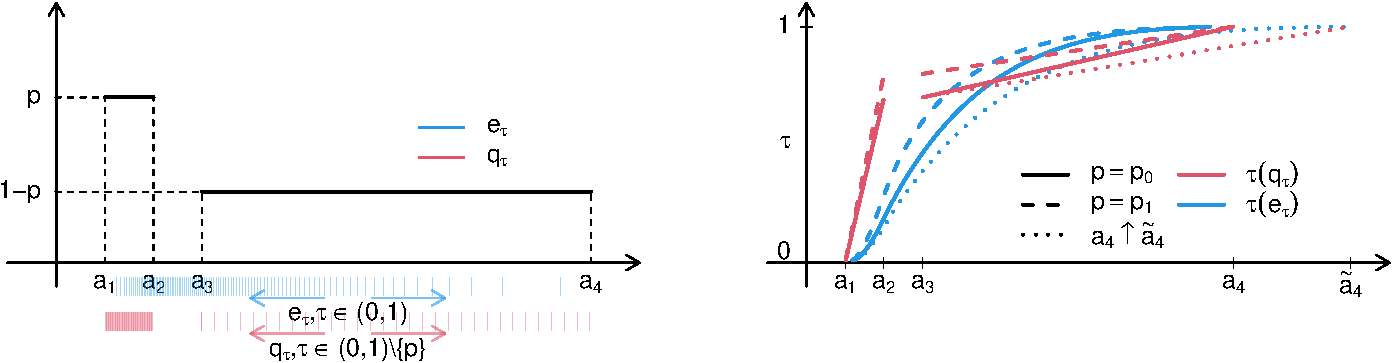
\includegraphics{paper_new_files/figure-latex/figexp1-1.pdf}
\caption{\label{fig:figexp1}Quantile and expectile functions for the mixture of two uniform distributions.}
\end{figure}

\begin{figure}
\centering
\includegraphics{paper_new_files/figure-latex/figexp12-1.pdf}
\caption{\label{fig:figexp12}Quantile and expectile functions for two scenarios of mixing parameter \(p\) in the mixture of two uniform distributions.}
\end{figure}

Figure \ref{fig:figexp12} illustrates the change in expectile function when \(p\) changes.
For mixtures of \(m\) disjoint (sorted) uniforms holds with mixing parameter vector \(\mathbf p=(p_1,\ldots,p_m)^\top\) where \(p_m=1-\sum_{i=1}^{m-1}p_i\) and support edges \(a_1<a_2<\ldots<a_{m+1}\):

\[\tau(e_\tau) = 
\begin{cases}
0,&e_\tau<a_1,\\
\frac{-\frac 12\frac{p_1}{a_2-a_1}(a_1-e_\tau)^2}  {-\frac{p_1}{a_2-a_1}(a_1-e_\tau)^2- \sum_{j=1}^mp_j\frac{a_{j+1}+a_j}2 +e_\tau} ,&a_1\leq e_\tau< a_2,\\
\frac{\frac 12\sum_{k=1}^{i-1}p_k\cdot (a_{k+1}+a_{k}-2e_\tau) -\frac 12 \cdot \frac{p_i}{a_{i+1}-a_i}(a_i-e_\tau)^2}  {\sum_{k=1}^{i-1}p_k\cdot (a_{k+1}+a_{k}-2e_\tau) -\frac{p_i}{a_{i+1}-a_i}(a_i-e_\tau)^2- \sum_{j=1}^mp_j\frac{a_{j+1}+a_j}2 +e_\tau} ,&a_i\leq e_\tau< a_{i+1},i=2,\ldots, m\\
1, &e_\tau\geq a_{m+1}.
\end{cases}\]

The derivations hereof are shown in the Appendix.
\end{example}

The problematic in Example \ref{exm:duqande} translates readily to the urban arterial roads travel times model of Zheng, Zuylen, and Liu (2017), where for the oversaturated condition, the probability function of delay consists of several box shaped functions with bounded support, which may (or may not) overlap. The authors distinguish two regimes: undersaturated and oversaturated conditions. The resulting delay distribution is composed of a mixture of Dirac delta function on fixed free-flow time (or a countinous distribution of free-flow time) and several uniform delay distributions with bounded support representing the effects of traffic lights, traffic control or similar conditions.

\begin{example}[Quantiles and expectiles of travel time distribution with discrete and continuous components]
\protect\hypertarget{exm:qdzheng}{}\label{exm:qdzheng}Consider now travel time distribution type proposed by Zheng, Zuylen, and Liu (2017), where there is a certain probability \(0<p_0<1\) of no delay so that the free flow travel time \(a_0\) is attained. In the same time, delays are possible and the delay distribution is a mixture of nonoverlapping uniform distributions with mixing parameter vector \(\mathbf p=(p_1,\ldots,p_m)^\top\) where \(p_m=1-\sum_{i=1}^{m-1}p_i-p_0\) and support edges \(a_1<a_2<\ldots<a_{m+1}\).

In this case the quantiles are well defined for \(i=1,\ldots, m\) and \(\tau\in(p_0,1)\setminus\{p_1,\ldots,p_m\}\) as:

\[q_\tau = a_{i} + \frac{a_{i+1}-a_{i}}{p_i}(\tau-\sum_{k=1}^{i-1}p_{k} - p_0), p_i<\tau<p_{i+1}.\]

The inverse expectile function is:

\[\tau(e_\tau) = 
\begin{cases}
0,&e_\tau<a_0,\\
(a_0-e_\tau)p_0,&a_0\leq e_\tau<a_1,\\
\frac{(a_0-e_\tau)p_0-\frac 12\frac{p_1}{a_2-a_1}(a_1-e_\tau)^2}  {(a_0-e_\tau)p_0-\frac{p_1}{a_2-a_1}(a_1-e_\tau)^2- \sum_{j=1}^mp_j\frac{a_{j+1}+a_j}2 +e_\tau} ,&a_1\leq e_\tau< a_2,\\
\frac{(a_0-e_\tau)p_0+\frac 12\sum_{k=1}^{i-1}p_k\cdot (a_{k+1}+a_{k}-2e_\tau) -\frac 12 \cdot \frac{p_i}{a_{i+1}-a_i}(a_i-e_\tau)^2}  {(a_0-e_\tau)p_0+\sum_{k=1}^{i-1}p_k\cdot (a_{k+1}+a_{k}-2e_\tau) -\frac{p_i}{a_{i+1}-a_i}(a_i-e_\tau)^2- \sum_{j=1}^mp_j\frac{a_{j+1}+a_j}2 +e_\tau} ,&a_i\leq e_\tau< a_{i+1},i=2,\ldots, m\\
1, &e_\tau\geq a_{m+1}.
\end{cases}\]
See Appendix for the derivation.

\begin{figure}
\centering
\includegraphics{paper_new_files/figure-latex/figexp2-1.pdf}
\caption{\label{fig:figexp2}Quantile and expectile functions for the mixture of a point mass and two uniform distributions.}
\end{figure}

For illustration purposes, we take over the setting of Example \ref{exm:duqande} with the only difference that we add \(a_0\) to the mixture with point probability \(p_0\). Figure \ref{fig:figexp2} illustrates the resulting departure time choices as quatiles (where uniquely defined) and expectiles of the mixture distribution.

In this example, we have a bunch of \(\tau\)-values, for which quantiles are not well defined. On the other hand, expectiles are still capable of capturing these kind of distributions.

As also explored in Zheng, Zuylen, and Liu (2017), the point mass at \(a_0\) can be substituted by a distribution centered at \(a_0\), since different vehicle or driver types may exhibit slightly varying free-flow times.
\end{example}

Note that instead of uniform mixture components, one can use more general forms offered for bounded supports e.g.~by four parameter beta distributions also used in Jabari, Freris, and Dilip (2020) for travel times modelling. In this case the form of \(\tau(e_\tau)\) becomes more complicated, however numeric computation based on Equation \eqref{eq:tau} is still feasible/possible.

Being quantile-alike tail indices, expectiles share some properties of quantiles, as location and scale equivariance.

\begin{proposition}[Location and scale equivariance of quantiles and expectiles]
\protect\hypertarget{prp:propprops}{}\label{prp:propprops}Let \(Y\in\mathbb R\) be a random variable with finite expectation, then for \(\tau \in (0,1)\) and \(s>0\)

\begin{itemize}
\item
  \(q_\tau(sY+m) = sq_\tau(Y) + m\) (follows from location and scale equivariance of the quantile loss function) and
\item
  \(e_\tau(sY+m)=se_\tau(Y) + m\) (Theorem 1 in Newey and Powell (1987)).
\end{itemize}

with \(\tau=\frac{\gamma}{\gamma+\beta}.\)
\end{proposition}

These properties are also useful for analysing the role of travel time mean and variance for optimal departure time plans.

Another useful property is the existence of the correspondence between (well defined) quantiles and expectiles (see Jones (1994), Yao and Tong (1996) and Waltrup et al. (2015)) of a distribution.

\begin{proposition}[Quantile-expectile correspondence]
\protect\hypertarget{prp:corr}{}\label{prp:corr}For each well defined \(\tau_1\)-quantile, there exist \(\tau_2(\tau_1)\in(0,1)\), such that \(q_{\tau_1}(Y) = e_{\tau_2(\tau_1)}(Y).\)
The correspondence function between quantile and expectiles of a random Variable \(T\in \mathbb R\) with distribution function \(F\), \(\tau_2(\tau_1):(0,1)\rightarrow(0,1)\) is:
\[\tau_2 (\tau_1) = \frac{-q_{\tau_1}\tau_1 + G(q_{\tau_1})}{-\mathbb EY + 2G(q_{\tau_1})+q_{\tau_1}(1-2\tau_1)},\]
where \(G(q) = \int_{-\infty}^qt~dF(t)\) is the partial moment function\footnote{Yao and Tong (1996) proof the result in the regression context.}.
\end{proposition}

\begin{proof}
For any distribution \(F\) with finite mean, the expectile function \(\tau_2\rightarrow e_{\tau_2}(F)\) is continuos, stricktly increasing and has range \(\{y\in\mathbb R: 0<F(y)<1\}\). So for each well defined quantile \(q_{\tau_1}=F^{-1}(\tau_1)\) there exists \(\tau_2\) such that
\[q_{\tau_1}(F) = e_{\tau_2}(F).\]

Following Yao and Tong (1996) and using the following identity for \(\tau_2\):
\[\tau_2 = \frac{\mathbb E(|Y-e_{\tau_2}|\mathbf 1_{Y\leq e_{\tau_2}})}{\mathbb E(|Y-e_{\tau_2}|\mathbf 1_{Y\leq e_{\tau_2}}) + \mathbb E(|Y-e_{\tau_2}|\mathbf 1_{Y> e_{\tau_2}})},\]

we get
\[\tau_2 (\tau_1) = \frac{\mathbb E(|Y-q_{\tau_1}|\mathbf 1_{Y\leq q_{\tau_1}})}{\mathbb E(|Y-q_{\tau_1}|\mathbf 1_{Y\leq q_{\tau_1}}) + \mathbb E(|Y-q_{\tau_1}|\mathbf 1_{Y> q_{\tau_1}})}=\]

\[= \frac{-\mathbb E(Y\mathbf 1_{Y\leq q_{\tau_1}})+q_{\tau_1}\tau_1}{\mathbb E(Y\mathbf 1_{Y\leq q_{\tau_1}})-q_{\tau_1}\tau_1 + \mathbb E(Y\mathbf 1_{Y> q_{\tau_1}})-q_{\tau_1}(1-\tau_1)}=\]

\[= \frac{-\mathbb E(Y\mathbf 1_{Y\leq q_{\tau_1}})+q_{\tau_1}\tau_1}{\mathbb EY - 2\mathbb E(Y\mathbf 1_{Y\leq q_{\tau_1}})-q_{\tau_1}(1-2\tau_1)}.\]

Rewriting \(\mathbb E(Y\mathbf 1_{Y\leq q}) = G(q)\), we obtain

\[\tau_2 (\tau_1) = \frac{-q_{\tau_1}\tau_1 + G(q_{\tau_1})}{-\mathbb EY + 2G(q_{\tau_1})+q_{\tau_1}(1-2\tau_1)}.\]
\end{proof}

Using this correspondence between quantiles and expectiles, a comparison of the optimal plans for the two parameterizations of the utility function are straight forward.

\begin{example}[Correspondence between quantiles and expectiles]
\protect\hypertarget{exm:corrqe}{}\label{exm:corrqe}Consider \(T\) with the uniform mixture distribution as in \ref{exm:qande}. The correspondence function between the associated \(\omega\)-quantile and the \(\tau\)-expectile of \(T\) \(\tau(\omega):(0,1)\setminus\{0.45\}\rightarrow(0,1)\) is
\[\tau(\omega)=\begin{cases}
\frac{-\omega q_\omega+ \frac 12 \frac p{a_2-a_1}(q_\omega^2-a_1^2)}{-\frac{p(a_1+a_2)}{2}-\frac{(1-p)(a_3+a_4)}{2} +\frac p{a_2-a_1}(q_\omega^2-a_1^2) + (1-2\omega)q_\omega},&q_\omega= a_1 + \frac{a_2-a_1} p\omega, \omega <p\\
\frac{-\omega q_\omega(T) + \frac 12 p(a_1+a_2) + \frac 12 \frac {1-p}{a_4-a_3}(q_\omega^2-a_3^2)}{-\frac{(1-p)(a_3+a_4)}{2} + \frac{p(a_1+a_2)}2 + \frac {1-p}{a_4-a_3}(q^2-a_3^2) + (1-2\omega)q_\omega},&q_\omega = a_3 + \frac{a_4-a_3}{1-p}(\omega-p), p<\omega
\end{cases}\]

and is shown in the Figure \ref{fig:figcor}.
\end{example}

\begin{figure}
\centering
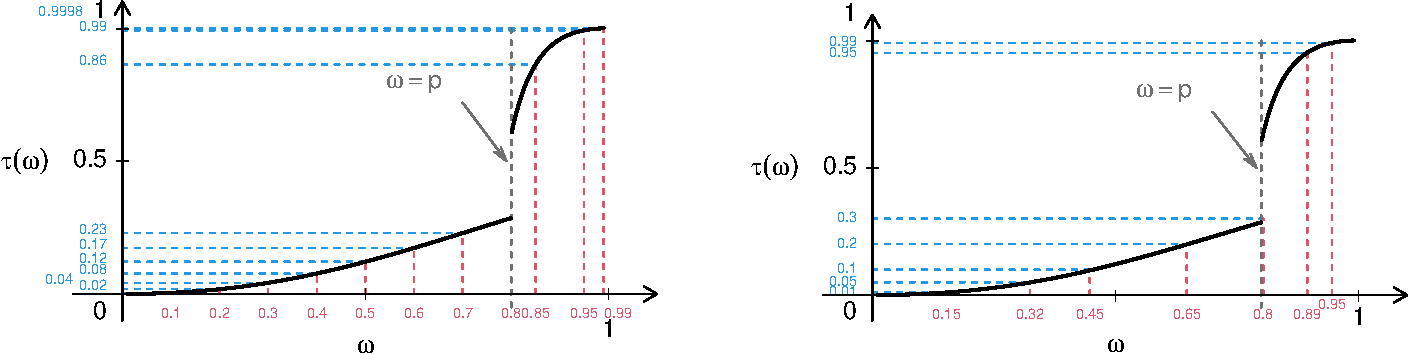
\includegraphics{paper_new_files/figure-latex/figcor-1.pdf}
\caption{\label{fig:figcor}Quantile- expectile correspondence function for mixture of two uniform distributions.}
\end{figure}

The sample counterparts, \(\hat q_\tau(X)\) and \(\hat e_\tau(X)\), of the population \(\tau\)-quantile and \(\tau\)-expectile are computed as plug-in estimators based on the empirical distribution function:

\begin{align}
\hat q_\tau(X) = \arg\min_{q\in\mathbb R}\sum_{i=1}^n||x_i-q||^1_{1,\tau}, \label{eq:q}
\end{align}
and

\begin{align}
\hat e_\tau(X) = \arg\min_{e\in\mathbb R}\sum_{i=1}^n||x_i-e||^2_{2,\tau}. \label{eq:e}
\end{align}

In this formulation, both are asymmetric versions of M-estimators, M-quantiles, and with the corresponding properties as consistency and under some more restrictive assumptions as finite second moment and continuous \(F\), asymptotic normality (Holzmann and Klar (2015), Abdous and Rémillard (1995), Breckling and Chambers (1988)). Moreover, as Abdous and Rémillard (1995), sample expectile estimators are more efficient than sample quantiles.

An estimate for the correspondence function can be obtained following the procedure of Taylor (2008), who construct an empirical cumulative distribution function by counting the observations below the estimated expectile for each of the \(\tau\)-levels, such that for each \(\tau\) there is a corresponding estimate of quantile index \(\omega\). One can then interpolate linearly between the resulting points to obtain \(\hat\tau(\omega)\).

\begin{example}[Sample quantiles and expectiles]
\protect\hypertarget{exm:qande}{}\label{exm:qande}

Consider a (ordered) sample of the ten travel times:

\[10.42, 12.46, 13.28, 14.53, 15.73, 16.78, 19, 19.55, 19.57, 101.16\]

generated from a mixture of two uniform distributions with mixing parameter \(p=0.9\) as well as \(a_1=10\), \(b_1=20\), \(a_2=30\), and \(b_2=110\).

For \(\tau \in\{0.1, 0.25, 0.5, 0.75, 0.9\}\)

\begin{itemize}
\item
  the sample quantiles are:
  \[\hat q_{0.1}=12.2568, \hat q_{0.25}=13.5927,\hat q_{0.5}=16.251,\hat q_{0.75}=19.4083,\hat q_{0.9}=27.7278\]
\item
  the sample expectiles are:
  \[\hat e_{0.1}=15.4291, \hat e_{0.25}=18.5847,\hat e_{0.5}=24.2471,\hat e_{0.75}=37.0664,\hat e_{0.9}=58.432\]
\end{itemize}

\end{example}

\hypertarget{quantiles-and-expectiles-of-travel-time-distribution-as-maximizers-of-u_1dt-and-u_2dt}{%
\subsection{\texorpdfstring{Quantiles and expectiles of travel time distribution as maximizers of \(U_1(d,T)\) and \(U_2(d,T)\)}{Quantiles and expectiles of travel time distribution as maximizers of U\_1(d,T) and U\_2(d,T)}}\label{quantiles-and-expectiles-of-travel-time-distribution-as-maximizers-of-u_1dt-and-u_2dt}}

Now, we come back to our planer's utility function in the asymmetric linear and quadratic versions. The following proposition connects the optimal departure times to quantiles and expectiles of travel time distribution.

\begin{proposition}[Optimal departure time plans]
\protect\hypertarget{prp:proputil}{}\label{prp:proputil}Let \(U_a(d,T), a\in\{1,2\}\) be planers utility function with \(\beta_a>0\) and \(\gamma_a>0\) fixed. Let \(T\) be random travel time with distribution function \(F\). Then, optimal departure time \(d^*\) corresponds to:

\begin{itemize}
\item
  the \(\tau_1\)-quantile \(q_{\tau_1}(T)\) of \(F\) in case of \(U_1(d,T)\)
\item
  the \(\tau_2\)-expectile \(e_{\tau_2}(T)\) of \(F\) in case of \(U_2(d,T)\)
\end{itemize}

with \(\tau_a=\frac{\gamma_a}{\gamma_a+\beta_a}\) and \(a\in\{1,2\}\). Alternatively, we can express the ratio \(\frac{\gamma_a}{\beta_a}\) in terms of \(\tau_a\) as \(\frac{\gamma_a}{\beta_a} = \frac{\tau_a}{1-\tau_a}.\)
\end{proposition}

\begin{proof}
Rewrite \(\mathbb EU_a(d,T)\) as
\[\mathbb EU_a(d,T) = -\left[\alpha_a \mathbb E(T^a) + (\gamma_a+\beta_a)\mathbb E\left\{\frac{\beta_a}{\gamma_a+\beta_a}(d-T)^a\mathbf 1_{T<d}+ \frac{\gamma_a}{\gamma_a+\beta_a}(T-d)^a\mathbf 1_{T\geq d}\right\}\right]\]

Setting \(\tau_a=\frac{\gamma_a}{\gamma_a+\beta_a}\) we get

\begin{align}
\mathbb EU_a(d,T) &= -\left[\alpha_a \mathbb E(T^a) + (\gamma_a+\beta_a)\mathbb E\left\{(1-\tau_a)(d-T)^a\mathbf 1_{T<d}+ \tau_a(T-d)^a\mathbf 1_{T\geq d}\right\}\right]\nonumber\\
&= -\left(\alpha_a \mathbb E(T^a) + (\gamma_a+\beta_a)\mathbb E\left[|T-d|^a\{(1-\tau_a)\mathbf 1_{T<d}+ \tau_a\mathbf 1_{T\geq d}\right\}\right)\nonumber\\
&= -\alpha_a \mathbb E(T^a) - (\gamma_a+\beta_a)\mathbb E||T-d||_{a,\tau_a}^a, \label{eq:as}
\end{align}
where, again, \(\tau_a = \frac{\gamma_a}{\beta_a+\gamma_a}\). That is, maximizing \(\mathbb EU_a(d,T)\) over \(d\in\mathbb R\) is equivalent to minimizing \(\mathbb E||T-d||_{a,\tau_a}^a\) which gives \(q_{\tau_1}(T)\) in case \(a=1\) and \(e_{\tau_2}(T)\) in case \(a=2\).
\end{proof}

Giving the optimal choice (\(d_1^*= q_{\tau_1}(T)\) or \(d_2^*= e_{\tau_2}(T)\)) the second term in \eqref{eq:as} corresponds to the asymmetric generalization of the absolute deviation (\(a=1\)) or of the variance (\(a=2\)) of random travel times. As a result, we get the \(\tau\)-deviation and the \(\tau\)-variance of \(T\), (\(Dev_\tau(T)\) and \(Var_\tau(T)\)), defined in Tran et al. (2019) as

\begin{equation}
Dev_\tau(T) = \mathbb E ||T-q_{\tau_1}(T)||_{1,\tau_1} \label{eq:tdev}
\end{equation}

and
\begin{equation}
Var_\tau(T) = \mathbb E ||T-e_{\tau_2}(T)||^2_{2,\tau_2}. \label{eq:tvar}
\end{equation}

Moreover, using the location scale invariance of quantiles in Proposition \ref{prp:propprops} in case of \(a=1\), we get the well known result of Fosgerau and Karlström (2010), where the optimal departure time \(d_1^* = \mu + \sigma F^{-1}\left(\frac{\gamma_1}{\beta_1+\gamma_1}\right)\) with \(F\) being the cumulative distribution function of the standardized travel time.

The result for \(a=2\) is new. Proposition \ref{prp:proputil} generalizes therefore the result of Fosgerau and Karlström (2010) to \(a\in\{1,2\}\) and provides a unified understanding of how the considered type of utility function is linked to the distributional properties of travel time \(T\).

As mentioned previously, there exist the correspondence function between quantiles and expectiles of a given distribution, which maps each well defined quantile \(q_{\alpha}(T)\) to an expectile \(e_{\tau(\alpha)}(T)\). Therefore, maximization of the expected utility in \eqref{eq:eu2} can produce the same choices for suitably chosen preference parameter \(\gamma/\beta\), see proposition \ref{prp:proputil2} below. Moreover, the asymmetric quadratic preference class is much richer than the asymmetric linear one as it delivers well defined solutions for every combination of scheduling preference parameters not only for distributions of \(T\) with strictly increasing \(F\) but also for discrete distributions or distribution with discontinuous support (see examples \ref{exm:ddqande} and \ref{exm:duqande}).

\begin{proposition}[Correspondence between $U_1$- and $U_2$-based choices]
\protect\hypertarget{prp:proputil2}{}\label{prp:proputil2}Let \(U_1(d,T)\) be planers utility function with known \(\gamma_1>\beta_1>0\). Let \(T\) be random travel time with distribution function \(F\) and finite mean. Then, for each \(\tau_1 = \frac{\gamma_1}{\beta_1+\gamma_1}\), in which \(F\) is invertible, there exist \(\tau_2\) and \(\gamma_2>\beta_2>0\) such that maximizing \(\mathbb E U_1(d,T)\) with respect to \(d\) is equivalent to maximizing \(\mathbb E U_2(d,T)\) with respect to \(d\) and thus both utilities represent the same scheduling preferences as they produce the same choices in the expected utility sense.
\end{proposition}

\begin{proof}
From \ref{prp:proputil} the optimal departure plan \(d_1^*\) for \(U_1(d,T)\) sattisfies:

\[d_1^* = \arg\min_{d\in \mathbb R^+}\mathbb E\left(||T-d||_{1,\tau_1}\right),\]

which matches with the \(\tau_1\)-quantile of travel time \(T\) with \(\tau_1=\frac{\gamma_1}{\beta_1+\gamma_1}\). Wenn \(F\) is invertible in \(\tau_1\), there exist a map \(\tau_2\equiv\tau_2(\tau_1)\) such that for the \(\tau_2\)-expectile, \(e_{\tau_2}\), holds \(e_{\tau_2} = q_{\tau_1}\). That is,

\[d_1^* = \arg\min_{d\in \mathbb R^+}\mathbb E\left(||T-d||_{1,\tau_1}\right) = \arg\min_{d\in \mathbb R^+}\mathbb E\left(||T-d||_{2,\tau_2}^2\right) = d_2^*.\]

The parameter \(\gamma_2>\beta_2>0\) are related as:

\begin{equation}\frac{\gamma_2}{\beta_2+\gamma_2} = \tau_2(\tau_1) = \tau_2\left(\frac{\gamma_1}{\beta_1+\gamma_1}\right), \label{eq:tcor}
\end{equation}

or \(\frac{\gamma_2}{\beta_2} = \frac{\tau_2}{1-\tau_2},\) where \(\tau_2\equiv \tau_2\left(\frac{\gamma_1}{\beta_1+\gamma_1}\right)\) is the quantile-expectile correspondence relation.
\end{proof}

\begin{example}[Optimal departure times for the sample of 10 travel times]
\protect\hypertarget{exm:optd}{}\label{exm:optd}

cont. of Example @ref(exm: qande). Comming back to our example with a sample of 10 travel times, we can now compute the optimal departure time points in the following example (see Table \ref{tab:table1}). We observe, that for smaller \(\gamma/\beta\)-ratios \(d_1^*\) is smaller than \(d_2^*\) and vice versa for larger \(\gamma/\beta\)-ratios.

\begin{table}

\caption{\label{tab:table1}Optimal $d^*$ for $U_1(d,T)$ and $U_2(d,T)$ based on the sample of the ten travel times: 10.42, 12.46, 13.28, 14.53, 15.73, 16.78, 19, 19.55, 19.57, 101.16.}
\centering
\begin{tabular}[t]{l|l|l|l|l|l|l|l|l}
\hline
  & \$\textbackslash{}frac\{\textbackslash{}beta\}\{\textbackslash{}gamma\}=1\$ & \$\textbackslash{}frac\{\textbackslash{}beta\}\{\textbackslash{}gamma\}=2\$ & \$\textbackslash{}frac\{\textbackslash{}beta\}\{\textbackslash{}gamma\}=3\$ & \$\textbackslash{}frac\{\textbackslash{}beta\}\{\textbackslash{}gamma\}=4\$ & \textbackslash{}frac\{\textbackslash{}beta\}\{\textbackslash{}gamma\}=9 & \textbackslash{}frac\{\textbackslash{}beta\}\{\textbackslash{}gamma\}=20 & \textbackslash{}frac\{\textbackslash{}beta\}\{\textbackslash{}gamma\}=50 & \textbackslash{}frac\{\textbackslash{}beta\}\{\textbackslash{}gamma\}=100\\
\hline
\$d\textasciicircum{}*\$ for \$U\_1(d,t)\$ & 16.25 & 19.00 & 19.41 & 19.55 & 27.73 & 66.19 & 86.76 & 93.89\\
\hline
\$d\textasciicircum{}*\$ for \$U\_2(d,t)\$ & 24.25 & 31.24 & 37.07 & 42.00 & 58.43 & 74.64 & 88.13 & 94.11\\
\hline
\end{tabular}
\end{table}

If we add another extreme travel time observation 87.67 to our sample, all expectiles alias \(d^*_2\) change substantially, whereas noticeable changes apply only to the higher quantiles (see Table \ref{tab:table3}). Though experiencing one more extreme travel time is likely to change the optimal departure plan for all types of planers.

\begin{table}

\caption{\label{tab:table3}Optimal $d^*$ for $U_1(d,T)$ and $U_2(d,T)$ based on the sample of the ten travel times: 10.42, 12.46, 13.28, 14.53, 15.73, 16.78, 19, 19.55, 19.57, 87.67, 101.16.}
\centering
\begin{tabular}[t]{l|l|l|l|l|l|l|l|l}
\hline
  & \$\textbackslash{}frac\{\textbackslash{}beta\}\{\textbackslash{}gamma\}=1\$ & \$\textbackslash{}frac\{\textbackslash{}beta\}\{\textbackslash{}gamma\}=2\$ & \$\textbackslash{}frac\{\textbackslash{}beta\}\{\textbackslash{}gamma\}=3\$ & \$\textbackslash{}frac\{\textbackslash{}beta\}\{\textbackslash{}gamma\}=4\$ & \textbackslash{}frac\{\textbackslash{}beta\}\{\textbackslash{}gamma\}=9 & \textbackslash{}frac\{\textbackslash{}beta\}\{\textbackslash{}gamma\}=20 & \textbackslash{}frac\{\textbackslash{}beta\}\{\textbackslash{}gamma\}=50 & \textbackslash{}frac\{\textbackslash{}beta\}\{\textbackslash{}gamma\}=100\\
\hline
\$d\textasciicircum{}*\$ for \$U\_1(d,t)\$ & 16.78 & 19.36 & 19.56 & 19.57 & 87.67 & 94.74 & 98.52 & 99.83\\
\hline
\$d\textasciicircum{}*\$ for \$U\_2(d,t)\$ & 30.01 & 39.92 & 47.19 & 52.74 & 68.18 & 79.96 & 88.12 & 94.05\\
\hline
\end{tabular}
\end{table}

\end{example}

In summary, the considered scheduling utility functions share the property, that maximizers of the resulting expected utilities are the tail indices (the \(\tau\)-quantile or the \(\tau\)-expectile) of random travel time, where the index \(\tau\) depends on the preference parameters (\(\tau=\gamma/(\beta+\gamma)\)). Moreover, via the quantile-expectile correspondence, a maximizer of \(\mathbb EU_2(d,t)\) is also a maximizer of \(\mathbb EU_1(d,t)\) for some corresponding preference transformation \(\tilde\gamma/\tilde \beta\) obtained by inversion of \eqref{eq:tcor} in case that the relevant \(\tau_1\)-quantile is unique. Hence, the choices induced by maximizing \eqref{eq:eu1} are a subset of the choices induced by \eqref{eq:eu2}, and the later enables a richer preference representation.

\hypertarget{quantifying-travel-time-reliability-under-asymmetric-scheduling-preferences}{%
\subsection{Quantifying travel time reliability under asymmetric scheduling preferences}\label{quantifying-travel-time-reliability-under-asymmetric-scheduling-preferences}}

We employ travel time reliability ratio (TTRR), denoted here as \(\rho_a\), for quantifiying travel time reliability. This ratio relates the value of travel time variability and to the value of travel time and is a commonly used measure in the literature (see Zang et al. (2022) and the references therein). Formally:

\begin{align}
\rho_a = \frac{d\mathbb EU_a^*}{d\sigma_T}/\frac{d\mathbb EU_a^*}{d\mu_T}, \label{eq:rho}
\end{align}

where \(\mu_T\) and \(\sigma_T\) refer to the mean and the standard deviation of \(T\).

Based on the results of Fosgerau and Karlström (2010) where

\begin{align}
\rho_1 = \frac{d\mathbb EU_1^*}{d\sigma_T}/\frac{d\mathbb EU_1^*}{d\mu_T} = \frac{\beta+\gamma}{\alpha}\int_{\frac{\gamma}{\beta+\gamma}}^1 F^{-1}(p)dp,
\label{eq:rho11}
\end{align}

Li (2019) propose a procedure to compute \eqref{eq:rho11} based on the conditional value at risk. Here we derive the expressions for \(\rho_a\) based on our notion of \(\mathbb EU_a(d,T)\) and propose an estimation procedure based on empirical partial moments.

\begin{proposition}[Travel time reliability ratio]
\protect\hypertarget{prp:proprho}{}\label{prp:proprho}Let \(U_a(d,T), a\in\{1,2\}\) be planers utility function with \(\beta>0\) and \(\gamma>0\) known. Let \(T\) be random travel time with distribution function \(F\) with finite mean \(\mu_T\) and finite variance \(\sigma_T^2\). Then, the travel time reliabilty ratio \(\rho_a\) is determined as:

\[\rho_a = \frac{a(\gamma+\beta)}{\alpha}\sigma_T^{a-1}\mathbb E||T_S-h_{a,\tau_a}(T_S)||_{a,\tau}^a,\]

with \(h_{a,\tau} = \begin{cases} q_\tau(T),&\text{for } a=1,\\ e_\tau(T),&\text{for }a=2.\end{cases}\) and \(\tau = \frac{\gamma}{\beta+\gamma}\).
\end{proposition}

\begin{proof}
Since \(\mathbb E(T^2) = \sigma_T^2 + \mu_T^2\), we can rerwrite \(\mathbb E(T^a) = \mu_T^{a} + (\sigma_T^2)^{a-1}\) and
\[\mathbb E U_a^*(d,T) =-\alpha (\mu_T^{a} + (\sigma_T^2)^{a-1}) - (\gamma+\beta)\mathbb E||T-h_{a,\tau}(T)||_{a,\tau}^a\\
=-\alpha (\mu_T^{a} + (\sigma_T^2)^{a-1})- (\gamma+\beta)\sigma_T^a\mathbb E||T_S-h_{a,\tau}(T_S)||_{a,\tau}^a\]

The last line based on the scale variance of expectiles and
\[\mathbb E||T-h_{a,\tau}(T)||_{a,\tau}^a=\mathbb E||(\sigma_TT_S + \mu_T)-(\sigma_Th_{a,\tau}(T_S)+\mu_T)||_{a,\tau}^a \\
= \mathbb E||\sigma_T(T_S-h_{a,\tau}(T_S))||_{a,\tau}^a = \sigma_T^a\mathbb E||T_S-h_{a,\tau^*}(T_S)||_{a,\tau}^a,\]

where \(T_S\) denotes the standardized version of \(T\). The value of travel time is:
\[\frac{d\mathbb EU_a^*}{d\mu_T} = -a\alpha \mu_T^{a-1} \]
The value of travel time variability is:
\[\frac{d\mathbb EU_a^*}{d\sigma_T} = -a(\gamma+\beta)\sigma_T^{a-1}\mathbb E||T_S-h_{a,\tau}(T_S)||_{a,\tau}^a\]
Thus,
\[\rho_a=\frac{a(\gamma+\beta)}{\alpha}\sigma_T^{a-1}\mathbb E||T_S-h_{a,\tau}(T_S)||_{a,\tau}^a\].
\end{proof}

Note that for \(a=1\) we recover:
\begin{equation}\rho_1 = \frac{(\gamma+\beta)}{\alpha}\mathbb E||T_S-q_{\tau_1}(T_S)||_{1,\tau_1}. \label{eq:rho1}
\end{equation}

In case \(a=2\) TTRR becomes:
\begin{equation}\rho_2=\frac{2(\gamma+\beta)}{\alpha}\sigma_T\mathbb E||T_S-e_{\tau_2}(T_S)||_{2,\tau_2}^2, \label{eq:rho2}
\end{equation}

and thus, explicitly depends on standard deviation of \(T\).

The terms \(\mathbb E||T_S-q_{\tau_1}(T_S)||_{1,\tau_1}\) and \(\mathbb E||T_S-e_{\tau_2}(T_S)||_{2,\tau_2}^2\) represent respectively the \(\tau\)-deviation \(Dev_\tau(T)\) defined in \eqref{eq:tdev} and the \(\tau\)-variance \(Var_\tau(T)\) defined in \eqref{eq:tvar}. Both can be obtained in practice using their empirical counterparts:

\[\widehat{Dev_\tau} (T) = \frac 1n\sum_{i=1}^n |\tau^*- \mathbf 1_{t_{S,i}\leq q_{\tau^*}}|\cdot|t_{S,i}-\hat q_{\tau^*}|\]
and

\[\widehat{Var_\tau} (T) = \frac 1n\sum_{i=1}^n |\tau^*- \mathbf 1_{t_{S,i}\leq q_{\tau^*}}|\cdot |t_{S,i}-\hat q_{\tau^*}|^2\]
which are both readily calculated from sampled of travel times.

Whereas \eqref{eq:rho1} is problematic in situations where the respective quantiles are not well defined, an expectile based measure in \eqref{eq:rho2} is feasible for all distributions with finite mean and variance.

\hypertarget{comparing-optimal-departure-time-choices-under-u_1td-and-u_2td-for-montreal-travel-time-data}{%
\section{\texorpdfstring{Comparing optimal departure time choices under \(U_1(T,d)\) and \(U_2(T,d)\) for Montreal travel time data}{Comparing optimal departure time choices under U\_1(T,d) and U\_2(T,d) for Montreal travel time data}}\label{comparing-optimal-departure-time-choices-under-u_1td-and-u_2td-for-montreal-travel-time-data}}

We provide a real data example using the dataset of travel times for Montreal.\footnote{ Available at
https://donnees.montreal.ca/dataset/temps-de-parcours-sur-des-segments-routiers-historique, accessed on 01 Jul 2023.} We take a subset of the data measures on link with ID 174in February 2019 6:00 and 7:00 am on regular working days Monday through Thursday. As suggested by kernel density estimate on Figure \ref{fig:figden}, the data semm to be generated by a model with several regimes. We, therefore model the data with a three component mixture of four-parameter beta distributions.

\begin{figure}
\centering
\includegraphics{paper_new_files/figure-latex/figden-1.pdf}
\caption{\label{fig:figden}Kernel density estimate for the considered travel times using authomatically chosen bandwidth 0.109.}
\end{figure}

Following the hybrid algorithm of Schröder and Rahmann (2016), who derives an iterative algorithm based on method of moments estimator, we estimate the parameters of the three component mixture distribution with bets components. The resulting estimates are presented in Table \ref{tab:tabpars}. Note, that the estimated mixture shows a gap in support and we expect, therefore, that the optimal departure time choice based on the estimated model will be non-unique in case of \(U_1\) with a certain preference combination \(\tau = \frac{\gamma}{\beta+\gamma}\).

\begin{table}

\caption{\label{tab:tabpars}The estimated parameters of the three component beta mixtures.}
\centering
\begin{tabular}[t]{l|l|l|l|l|l}
\hline
  & probability & shape 1 & shape 2 & lower & upper\\
\hline
component 1 & 0.775 & 0.88 & 1.33 & 0.58 & 2.01\\
\hline
component 2 & 0.224 & 0.74 & 6.15 & 1.99 & 11.00\\
\hline
component 3 & 0.001 & 0.65 & 3.04 & 14.07 & 31.16\\
\hline
\end{tabular}
\end{table}

Note, that there is a gap in the support of the estimated mixture between second and third component on the interval \((11,14.07)\). That is, for the \(\tau\)-value equal to the cumulative probability of the first two components, there will be no unique value.

\begin{figure}
\centering
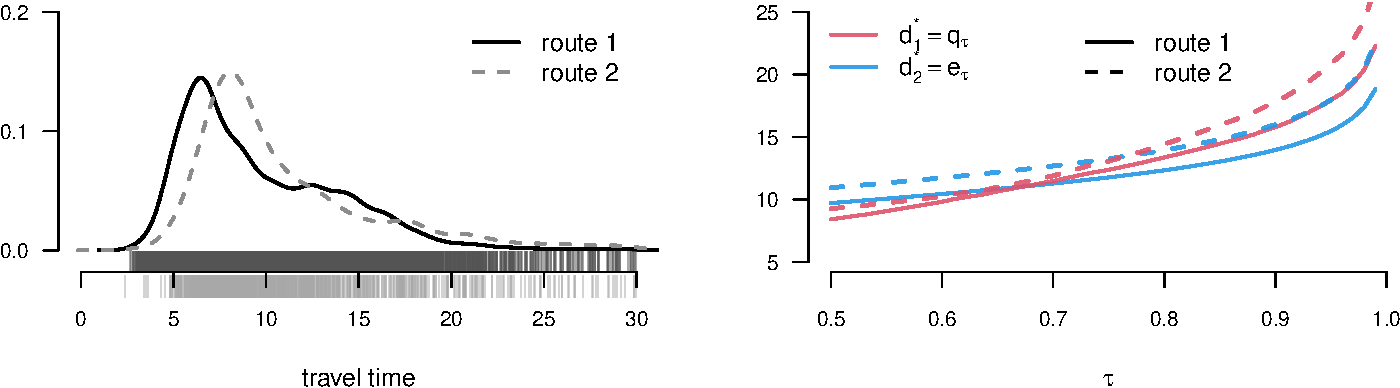
\includegraphics{paper_new_files/figure-latex/choices-1.pdf}
\caption{\label{fig:choices}Left panel: the optimal choices as quantiles (when uniquely defined) for \(U_1\) and expectiles for \(U_2\) and different preference specification \$ au\$. Right panel: the section on the support, where the quantile for \$ au=0.999\$ is non-unique.}
\end{figure}

Hence, for this real data example, the optimal departure plan for a planer with \(U_1\) and preference parameters which yield \(\tau=0.999\), no unique solution can be found as any value on the interval \((11,14.07)\) is admissible. Whereas, for a planer with \(U_2\) the choice is unique, no matter which preference parameters she has.

The corresponding optimal departure time choices for both utility types are plotted in Figure \ref{fig:choices}. On the left panel, we show the optimal choices as quantiles (when uniquely defined) for \(U_1\) and expectiles for \(U_2\) and different preference scpecification \(\tau=\frac{\gamma}{\beta+\gamma}\). On the right plot of Figure \ref{fig:choices}, we ``zoom in'' to the interval near \(\tau=0.999\).

In this example, we have the following quantile-expectile correspondence \(\tau_2(\tau_1)\) for \(\tau_1\in(0.5,1)\) with a ``hole'' at \(\tau_1=0.999\) which is show in Figure \ref{fig:figcor2}.

Finally, the variability measures and the TTRRs as functions of \(\tau\) are plotted in Figure .

\begin{figure}
\centering
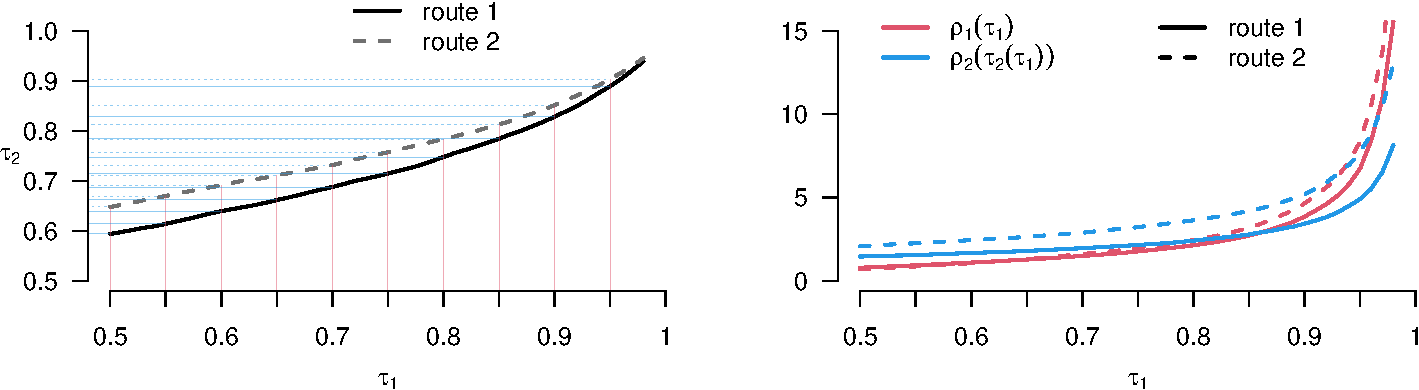
\includegraphics{paper_new_files/figure-latex/figcor2-1.pdf}
\caption{\label{fig:figcor2}Left panel: the estimated quantile-expectile correspondece for the considerred travel time data. Right panel: the derived TTRRs for both utility specifications and the considerred travel time data.}
\end{figure}

As seen, the value of travel time reliability associated with \(U_2\) is always higher than that of \(U_1\) for the same preference parameterization \(\beta/\gamma\).

\hypertarget{conclusion}{%
\section{Conclusion}\label{conclusion}}

In this paper, we considered a classical specification of scheduling utility as asymmetric linear function of delays along with a new alternative specification based on asymmetric quadratic loss. We showed that the optimal departure choices for both utilities are tail indices of travel time distribution. Specifically, for the asymmetric linear specification those are certain quantiles and for the asymmetric quadratic specification, expectiles, of the travel time. Moreover, we demonstrated that there exists a correspondence of choices based on our alternative specification to the choices made according to the classical one in case of invertible cumulative distribution function. Finally, we show that our asymmetric quadratic preference formulation is a richer one, since unique optimum is obtained for any distribution of travel time with finite mean. Using the travel time data collected in Montreal, we empirically demonstrated the advantages of using the second utility specification.

\hypertarget{appendix}{%
\section{Appendix}\label{appendix}}

\hypertarget{deriviations-in-example-refexmduqande}{%
\subsection{Deriviations in Example \ref{exm:duqande}}\label{deriviations-in-example-refexmduqande}}

For a mixure of \(m\) nonoverlapping uniforms (disjoint supports) with mixing parameter vector \(\mathbf p=(p_1,\ldots,p_m)^\top\) where \(p_m=1-\sum_{i=1}^{m-1}p_i\) and support edges \(a_1<a_2<\ldots<a_m\):
\[f(y)=\sum_{j=1}^m\frac{p_j}{a_{j+1}-a_j}\mathbf 1_{y\in [a_j,a_{j+1}]}.\]

The inverse expectile function is defined as:

\begin{equation}\tau(e_\tau) = \frac{\mathbb E\{(Y-e_\tau)\mathbf 1_{Y\leq e_\tau}\}}  {2\mathbb E\{(Y-e_\tau)\mathbf 1_{Y\leq e_\tau}\} - \mathbb E\{(Y-e_\tau)\}}\end{equation}

For \(\mathbb E\{(Y-e_\tau)\mathbf 1_{Y\leq e_\tau}\}\) we have:

\begin{itemize}
\tightlist
\item
  for \(a_1\leq e_\tau< a_2\)
\end{itemize}

\[\mathbb E\{(Y-e_\tau)\mathbf 1_{Y\leq e_\tau}\} = \int_{a_1}^{e_\tau}(y-e_\tau)\frac{p_1}{a_2-a_1}dy = \frac{p_1}{a_2-a_1}\int_{a_1}^{e_\tau}(y-e_\tau)dy\]

\[ = \frac{p_1}{a_2-a_1}\frac 12[(y-e_\tau)^2]_{a_1}^{e_\tau} = -\frac{p_1}{a_2-a_1}\frac 12 (a_1-e_\tau)^2\]

\begin{itemize}
\tightlist
\item
  for \(a_2\leq e_\tau< a_3\)
\end{itemize}

\[\mathbb E\{(Y-e_\tau)\mathbf 1_{Y\leq e_\tau}\} = \int_{a_1}^{a_2}(y-e_\tau)\frac{p_1}{a_2-a_1}dy + \int_{a_2}^{e_\tau}(y-e_\tau)\frac{p_2}{a_3-a_2}dy\]

\[ = \frac{p_1}{a_2-a_1}\frac 12[(y-e_\tau)^2]_{a_1}^{a_2} + \frac{p_2}{a_3-a_2}\frac 12[(y-e_\tau)^2]_{a_2}^{e_\tau} =\frac{p_1}2\cdot (a_2+a_1-2e_\tau) -\frac{p_2}{a_3-a_2}\frac 12 (a_2-e_\tau)^2\]

\begin{itemize}
\tightlist
\item
  for \(a_i\leq e_\tau< a_{i+1}, 1<i\leq m\)
\end{itemize}

\[\mathbb E\{(Y-e_\tau)\mathbf 1_{Y\leq e_\tau}\} =\int_{a_1}^{a_{i}}(y-e_\tau)f(y)dy +  \int_{a_i}^{e_\tau}(y-e_\tau)f(y)dy\]
\[=\sum_{k=1}^{i-1}\frac{p_k}{a_{k+1}-a_k}\int_{a_k}^{a_{k+1}}(y-e_\tau)dy + \frac{p_i}{a_{i+1}-a_i} \int_{a_i}^{e_\tau}(y-e_\tau)dy\]

\[=\frac 12\sum_{k=1}^{i-1}p_k\cdot (a_{k+1}+a_{k}-2e_\tau) -\frac 12 \cdot \frac{p_i}{a_{i+1}-a_i}(a_i-e_\tau)^2 =\left(\sum_{k=1}^{i-1}{p_k}\frac{a_{k+1}+a_{k}}2-p_ke_\tau\right) -\frac 12 \cdot \frac{p_i}{a_{i+1}-a_i}(a_i-e_\tau)^2 .\]
In the expression above, the first term represents the weighted mean-expectile difference of mixture components with supports below the \(i\)th component and the second term measures weighted expectation below \(e_\tau\) for the \(i\)th component.

Also,

\[\mathbb E(Y-e_\tau) =\sum_{j=1}^m\frac{p_j}{a_{j+1}-a_j}\int_{a_j}^{a_{j+1}}(y-e_\tau) dy = 
\sum_{j=1}^m\frac{p_j}2(a_{j+1}+a_j-2e_\tau)\]

Rearranged, we have
\[\mathbb E(Y-e_\tau)  = \sum_{j=1}^mp_j\frac{a_{j+1}+a_j}2 -e_\tau,\]
which represents the weighted mean of mixture components minus the \(\tau\)-expectile.

Hence,
\begin{equation}\tau(e_\tau) = \begin{cases}
0,&e_\tau<a_1,\\
\frac{-\frac 12\frac{p_1}{a_2-a_1}(a_1-e_\tau)^2}  {-\frac{p_1}{a_2-a_1}(a_1-e_\tau)^2- \sum_{j=1}^mp_j\frac{a_{j+1}+a_j}2 +e_\tau} ,&a_1\leq e_\tau< a_2,\\
\frac{\frac 12\sum_{k=1}^{i-1}p_k\cdot (a_{k+1}+a_{k}-2e_\tau) -\frac 12 \cdot \frac{p_i}{a_{i+1}-a_i}(a_i-e_\tau)^2}  {\sum_{k=1}^{i-1}p_k\cdot (a_{k+1}+a_{k}-2e_\tau) -\frac{p_i}{a_{i+1}-a_i}(a_i-e_\tau)^2- \sum_{j=1}^mp_j\frac{a_{j+1}+a_j}2 +e_\tau} ,&a_i\leq e_\tau< a_{i+1},i=2,\ldots, m\\
1, &e_\tau\geq a_{m+1}.
\end{cases}\end{equation}

\hypertarget{deriviations-in-example-refexmqdzheng}{%
\subsection{Deriviations in Example \ref{exm:qdzheng}}\label{deriviations-in-example-refexmqdzheng}}

For \(\mathbb E\{(Y-\mu_\tau)\mathbf 1_{Y\leq\mu_\tau}\}\) we have:

\begin{itemize}
\tightlist
\item
  for \(a_0\leq e_\tau< a_1\)
\end{itemize}

\[\mathbb E\{(Y-\mu_\tau)\mathbf 1_{Y\leq\mu_\tau}\} = (a_0-e_\tau)p_0.\]

Analogous to the previous example, we have

\begin{itemize}
\tightlist
\item
  for \(a_1\leq e_\tau< a_2\)
\end{itemize}

\[\mathbb E\{(Y-e_\tau)\mathbf 1_{Y\leq e_\tau}\} = (a_0-e_\tau)p_0 + \int_{a_1}^{e_\tau}(y-e_\tau)\frac{p_1}{a_2-a_1}dy\]
\[= (a_0-e_\tau)p_0 -\frac{p_1}{a_2-a_1}\frac 12 (a_1-e_\tau)^2\]

\begin{itemize}
\tightlist
\item
  for \(a_2\leq \mu_\tau< a_3\)
\end{itemize}

\[\mathbb E\{(Y-e_\tau)\mathbf 1_{Y\leq e_\tau}\} = (a_0-e_\tau)p_0 + \int_{a_1}^{a_2}(y-e_\tau)\frac{p_1}{a_2-a_1}dy + \int_{a_2}^{e_\tau}(y-\mu_\tau)\frac{p_2}{a_3-a_2}dy\]

\[ = (a_0-e_\tau)p_0+\frac{p_1}2\cdot (a_2+a_1-2 e_\tau) -\frac{p_2}{a_3-a_2}\frac 12 (a_2-e_\tau)^2\]

\begin{itemize}
\tightlist
\item
  for \(a_i\leq e_\tau< a_{i+1}, 1<i\leq m\)
\end{itemize}

\[\mathbb E\{(Y-e_\tau)\mathbf 1_{Y\leq e_\tau}\} =(a_0-e_\tau)p_0 + \int_{a_1}^{a_{i}}(y-e_\tau)f(y)dy +  \int_{a_i}^{\mu_\tau}(y-e_\tau)f(y)dy\]
\[=(a_0-e_\tau)p_0+ \sum_{k=1}^{i-1}\frac{p_k}{a_{k+1}-a_k}\int_{a_k}^{a_{k+1}}(y-e_\tau)dy + \frac{p_i}{a_{i+1}-a_i} \int_{a_i}^{e_\tau}(y-e_\tau)dy\]

\[=(a_0-e_\tau)p_0+ \frac 12\sum_{k=1}^{i-1}p_k\cdot (a_{k+1}+a_{k}-2e_\tau) -\frac 12 \cdot \frac{p_i}{a_{i+1}-a_i}(a_i-e_\tau)^2.\]

Also,

\[\mathbb E(Y-e_\tau) =(a_0-e_\tau)p_0 + \sum_{j=1}^m\frac{p_j}{a_{j+1}-a_j}\int_{a_j}^{a_{j+1}}(y-e_\tau) dy = \\
=(a_0-e_\tau)p_0+ \sum_{j=1}^m\frac{p_j}2(a_{j+1}+a_j-2 e_\tau)\]

Hence,
\begin{equation}\tau(\mu_\tau) = \begin{cases}
0,&e_\tau<a_0,\\
(a_0-e_\tau)p_0,&a_0\leq e_\tau<a_1,\\
\frac{(a_0-e_\tau)p_0-\frac 12\frac{p_1}{a_2-a_1}(a_1-e_\tau)^2}  {(a_0-e_\tau)p_0-\frac{p_1}{a_2-a_1}(a_1-e_\tau)^2- \sum_{j=1}^mp_j\frac{a_{j+1}+a_j}2 +e_\tau} ,&a_1\leq e_\tau< a_2,\\
\frac{(a_0-e_\tau)p_0+\frac 12\sum_{k=1}^{i-1}p_k\cdot (a_{k+1}+a_{k}-2e_\tau) -\frac 12 \cdot \frac{p_i}{a_{i+1}-a_i}(a_i-e_\tau)^2}  {(a_0-e_\tau)p_0+\sum_{k=1}^{i-1}p_k\cdot (a_{k+1}+a_{k}-2e_\tau) -\frac{p_i}{a_{i+1}-a_i}(a_i-e_\tau)^2- \sum_{j=1}^mp_j\frac{a_{j+1}+a_j}2 +e_\tau} ,&a_i\leq e_\tau< a_{i+1},i=2,\ldots, m\\
1, &e_\tau\geq a_{m+1}.
\end{cases}\end{equation}

\hypertarget{derivations-in-example-refexmcorrqe}{%
\subsection{Derivations in Example \ref{exm:corrqe}}\label{derivations-in-example-refexmcorrqe}}

\[\tau(\omega)=\frac{-\omega q_\omega(T) + G(q_\omega(T))}{-\mathbb ET - 2G(q_\omega(T)) + (1-2\omega)q_\omega(T)},\]

where \(G(q) = \int_{-\infty}^qt~dF(t)\)

We have
for \(\omega <p\), \(q_\omega= a_1 + \frac{a_2-a_1} p\omega\),
\[G(q) = \int_{a_1}^q t\cdot\frac p{a_2-a_1}dt = \frac 12 \frac p{a_2-a_1}(q^2-a_1^2)\]

and for \(p<\omega\), \(q_\omega = a_3 + \frac{a_4-a_3}{1-p}(\omega-p),\)
\[G(q) = \int_{a_1}^{a_2} t\cdot\frac p{a_2-a_1}dt + \int_{a_3}^q t\cdot\frac {1-p}{a_2-a_1}dt = \frac 12 p(a_1+a_2) + \frac 12 \frac {1-p}{a_4-a_3}(q^2-a_3^2)\]

So,

\[\tau(\omega)=\begin{cases}
\frac{-\omega q_\omega+ \frac 12 \frac p{a_2-a_1}(q_\omega^2-a_1^2)}{-\frac{p(a_1+a_2)}{2}-\frac{(1-p)(a_3+a_4)}{2} - \frac p{a_2-a_1}(q_\omega^2-a_1^2) + (1-2\omega)q_\omega},&q_\omega= a_1 + \frac{a_2-a_1} p\omega, \omega <p\\
\frac{-\omega q_\omega(T) + \frac 12 p(a_1+a_2) + \frac 12 \frac {1-p}{a_4-a_3}(q_\omega^2-a_3^2)}{-\frac{(1-p)(a_3+a_4)}{2} - \frac{3p(a_1+a_2)}2 - \frac {1-p}{a_4-a_3}(q^2-a_3^2) + (1-2\omega)q_\omega},&q_\omega = a_3 + \frac{a_4-a_3}{1-p}(\omega-p), p<\omega
\end{cases}.\]

TODO:

\begin{itemize}
\tightlist
\item
  add dashed lines to the empirical correspondence
\item
  check the tables and their positions
\item
  check the figures, scale
\item
  check indices, 1,2 notation or e(T) or mention that it is omitted where unambiguous.
\end{itemize}

\hypertarget{refs}{}
\begin{CSLReferences}{1}{0}
\leavevmode\vadjust pre{\hypertarget{ref-abdous1995}{}}%
Abdous, Belkacem, and Bruno N. Rémillard. 1995. {``Relating Quantiles and Expectiles Under Weighted-Symmetry.''} \emph{Annals of the Institute of Statistical Mathematics} 47: 371--84.

\leavevmode\vadjust pre{\hypertarget{ref-enide2006}{}}%
Bogers, Enide A. I., Francesco Viti, Serge P. Hoogendoorn, and Henk J. Van Zuylen. 2006. {``Valuation of Different Types of Travel Time Reliability in Route Choice: Large-Scale Laboratory Experiment.''} \emph{Transportation Research Record} 1985 (1): 162--70. \url{https://doi.org/10.1177/0361198106198500118}.

\leavevmode\vadjust pre{\hypertarget{ref-breckling1988}{}}%
Breckling, Jens, and Ray Chambers. 1988. {``M-Quantiles.''} \emph{Biometrika} 75 (4): 761--71. \url{https://doi.org/10.1093/biomet/75.4.761}.

\leavevmode\vadjust pre{\hypertarget{ref-daganzo1985}{}}%
Daganzo, Carlos F. 1985. {``The Uniqueness of a Time-Dependent Equilibrium Distribution of Arrivals at a Single Bottleneck.''} \emph{Transportation Science} 19 (1): 29--37. \url{https://doi.org/10.1287/trsc.19.1.29}.

\leavevmode\vadjust pre{\hypertarget{ref-depalma2012}{}}%
de Palma, André, Robin Lindsey, and Nathalie Picard. 2012. {``Risk Aversion, the Value of Information, and Traffic Equilibrium.''} \emph{Transportation Science} 46 (1): 1--26. \url{https://doi.org/10.1287/trsc.1110.0357}.

\leavevmode\vadjust pre{\hypertarget{ref-depalma2006}{}}%
de Palma, André, and Nathalie Picard. 2006. {``Equilibria and Information Provision in Risky Networks with Risk-Averse Drivers.''} \emph{Transportation Science} 40 (4): 393--408. \url{https://doi.org/10.1287/trsc.1060.0152}.

\leavevmode\vadjust pre{\hypertarget{ref-engelson2016}{}}%
Engelson, Leonid, and Mogens Fosgerau. 2016. {``The Cost of Travel Time Variability: Three Measures with Properties.''} \emph{Transportation Research Part B: Methodological} 91: 555--64. https://doi.org/\url{https://doi.org/10.1016/j.trb.2016.06.012}.

\leavevmode\vadjust pre{\hypertarget{ref-fosgerau2010}{}}%
Fosgerau, Mogens, and Anders Karlström. 2010. {``The Value of Reliability.''} \emph{Transportation Research Part B: Methodological} 44 (1): 38--49. https://doi.org/\url{https://doi.org/10.1016/j.trb.2009.05.002}.

\leavevmode\vadjust pre{\hypertarget{ref-guo2017}{}}%
Guo, Ren-Yong, Hai Yang, Hai-Jun Huang, and Xinwei Li. 2017. {``Day-to-Day Departure Time Choice Under Bounded Rationality in the Bottleneck Model.''} \emph{Transportation Research Part B: Methodological} 117 (September). \url{https://doi.org/10.1016/j.trb.2017.08.016}.

\leavevmode\vadjust pre{\hypertarget{ref-holzmann2016}{}}%
Holzmann, Hajo, and Bernhard Klar. 2015. {``Expectile Asymptotics.''} \emph{Electronic Journal of Statistics} 10 (September). \url{https://doi.org/10.1214/16-EJS1173}.

\leavevmode\vadjust pre{\hypertarget{ref-jabari2019}{}}%
Jabari, Saif Eddin, Nikolaos M. Freris, and Deepthi Mary Dilip. 2020. {``Sparse Travel Time Estimation from Streaming Data.''} \emph{Transportation Science} 54 (1): 1--20. \url{https://doi.org/10.1287/trsc.2019.0920}.

\leavevmode\vadjust pre{\hypertarget{ref-jackson1982}{}}%
Jackson, W. Burke, and James V. Jucker. 1982. {``An Empirical Study of Travel Time Variability and Travel Choice Behavior.''} \emph{Transportation Science} 16 (4): 460--75. \url{https://doi.org/10.1287/trsc.16.4.460}.

\leavevmode\vadjust pre{\hypertarget{ref-jin2020}{}}%
Jin, Wen-Long. 2020. {``Stable Day-to-Day Dynamics for Departure Time Choice.''} \emph{Transportation Science} 54 (1): 42--61. \url{https://doi.org/10.1287/trsc.2019.0919}.

\leavevmode\vadjust pre{\hypertarget{ref-jones1994}{}}%
Jones, M. C. 1994. {``Expectiles and m-Quantiles Are Quantiles.''} \emph{Statistics \& Probability Letters} 20 (2): 149--53. https://doi.org/\url{https://doi.org/10.1016/0167-7152(94)90031-0}.

\leavevmode\vadjust pre{\hypertarget{ref-koenker1978}{}}%
Koenker, Roger W, and Gilbert Bassett. 1978. {``Regression Quantiles.''} \emph{Econometrica} 46 (1): 33--50. \url{https://EconPapers.repec.org/RePEc:ecm:emetrp:v:46:y:1978:i:1:p:33-50}.

\leavevmode\vadjust pre{\hypertarget{ref-li2019}{}}%
Li, Baibing. 2019. {``Measuring Travel Time Reliability and Risk: A Nonparametric Approach.''} \emph{Transportation Research Part B: Methodological} 130: 152--71. https://doi.org/\url{https://doi.org/10.1016/j.trb.2019.10.009}.

\leavevmode\vadjust pre{\hypertarget{ref-lindsey2004}{}}%
Lindsey, Robin. 2004. {``Existence, Uniqueness, and Trip Cost Function Properties of User Equilibrium in the Bottleneck Model with Multiple User Classes.''} \emph{Transportation Science} 38 (3): 293--314. \url{https://doi.org/10.1287/trsc.1030.0045}.

\leavevmode\vadjust pre{\hypertarget{ref-newey1987}{}}%
Newey, Whitney, and James Powell. 1987. {``Asymmetric Least Squares Estimation and Testing.''} \emph{Econometrica} 55 (February): 819--47. \url{https://doi.org/10.2307/1911031}.

\leavevmode\vadjust pre{\hypertarget{ref-philipps2022}{}}%
Philipps, Collind. 2022. {``Interpreting Expectiles.''} \emph{Available at SSRN: Http://Dx.doi.org/10.2139/Ssrn.3881402}. https://doi.org/\url{http://dx.doi.org/10.2139/ssrn.3881402}.

\leavevmode\vadjust pre{\hypertarget{ref-schroeder2016}{}}%
Schröder, Christopher, and Sven Rahmann. 2016. {``A Hybrid Parameter Estimation Algorithm for Beta Mixtures and Applications to Methylation State Classification.''} In, 9838:307--19. \url{https://doi.org/10.1007/978-3-319-43681-4_25}.

\leavevmode\vadjust pre{\hypertarget{ref-small1982}{}}%
Small, Kenneth. 1982. {``The Scheduling of Consumer Activities: Work Trips.''} \emph{American Economic Review} 72 (February): 467--79.

\leavevmode\vadjust pre{\hypertarget{ref-small2015}{}}%
Small, Kenneth A. 2015. {``The Bottleneck Model: An Assessment and Interpretation.''} \emph{Economics of Transportation} 4 (1): 110--17. https://doi.org/\url{https://doi.org/10.1016/j.ecotra.2015.01.001}.

\leavevmode\vadjust pre{\hypertarget{ref-smith1984}{}}%
Smith, Michael J. 1984. {``The Existence of a Time-Dependent Equilibrium Distribution of Arrivals at a Single Bottleneck.''} \emph{Transportation Science} 18 (4): 385--94. \url{https://doi.org/10.1287/trsc.18.4.385}.

\leavevmode\vadjust pre{\hypertarget{ref-taylor2008}{}}%
Taylor, James W. 2008. {``{Estimating Value at Risk and Expected Shortfall Using Expectiles}.''} \emph{Journal of Financial Econometrics} 6 (2): 231--52. \url{https://doi.org/10.1093/jjfinec/nbn001}.

\leavevmode\vadjust pre{\hypertarget{ref-tran2019}{}}%
Tran, Ngoc M., Petra Burdejová, Maria Osipenko, and Wolfgang K. Härdle. 2019. {``Principal Component Analysis in an Asymmetric Norm.''} \emph{Journal of Multivariate Analysis} 171: 1--21. https://doi.org/\url{https://doi.org/10.1016/j.jmva.2018.10.004}.

\leavevmode\vadjust pre{\hypertarget{ref-waltrup2015}{}}%
Waltrup, Linda Schulze, Fabian Sobotka, Thomas Kneib, and Göran Kauermann. 2015. {``Expectile and Quantile Regression---David and Goliath?''} \emph{Statistical Modelling} 15 (5): 433--56. \url{https://doi.org/10.1177/1471082X14561155}.

\leavevmode\vadjust pre{\hypertarget{ref-yao1996}{}}%
Yao, Qiwli, and Howell Tong. 1996. {``Asymmetric Least Squares Regression Estimation: A Nonparametric Approach.''} \emph{Journal of Nonparametric Statistics} 6 (2-3): 273--92. \url{https://doi.org/10.1080/10485259608832675}.

\leavevmode\vadjust pre{\hypertarget{ref-zang2022}{}}%
Zang, Zhaoqi, Xiangdong Xu, Kai Qu, Ruiya Chen, and Anthony Chen. 2022. {``Travel Time Reliability in Transportation Networks: A Review of Methodological Developments.''} \emph{Transportation Research Part C: Emerging Technologies} 143: 103866. https://doi.org/\url{https://doi.org/10.1016/j.trc.2022.103866}.

\leavevmode\vadjust pre{\hypertarget{ref-zhang2016}{}}%
Zhang, Leilei, and Tito Homem-de-Mello. 2017. {``An Optimal Path Model for the Risk-Averse Traveler.''} \emph{Transportation Science} 51 (2): 518--35. \url{https://doi.org/10.1287/trsc.2016.0685}.

\leavevmode\vadjust pre{\hypertarget{ref-zheng_fangfang2017}{}}%
Zheng, Fangfang, Henk van Zuylen, and Xiaobo Liu. 2017. {``A Methodological Framework of Travel Time Distribution Estimation for Urban Signalized Arterial Roads.''} \emph{Transportation Science} 51 (3): 893--917. \url{https://doi.org/10.1287/trsc.2016.0718}.

\end{CSLReferences}

\end{document}
